\documentclass[11pt,a4paper]{article}

\usepackage{graphicx}
\usepackage[font=footnotesize]{caption}
\usepackage[noadjust]{cite}
\usepackage[toc,page]{appendix}
\usepackage{hyperref}
\usepackage{fullpage}
\usepackage{amsmath}
\usepackage{sidecap}
\usepackage{subcaption}
\usepackage{minted}
\usepackage{framed}


\renewcommand*\abstractname{Summary}

% OUR COMMANDS
%~ 
%~ \newenvironment{pythoncode}%
%~ {\begin{framed}
%~ \begin{minted}{python}}%
%~ {\end{minted}
%~ \end{framed}}%

% package name:
\newcommand{\means}{\texttt{MEANS}}
\newcommand{\pft}{\textit{p53}}
\newcommand{\py}{\texttt{python}}

\begin{document}
\title{MEANS: a new python package for Moment Expansion Approximation, Inference and Simulation}
\author{Sisi Fan, Quentin Geissmann, Saulius Lukauskas}
\date{\today}



\clearpage\maketitle
\thispagestyle{empty}
\newpage{}

\pagenumbering{roman}
\begin{abstract}
TODO An abstract here...
\end{abstract}

TODO ABREVIATIONS table!!
ODE 
MEA
TODO, make a bib entry for Lakatos, unpublished/in prep.

\tableofcontents


\newpage{}
\pagenumbering{arabic}
\section{Introduction} \label{intro}

Most biological systems, such as cells, organisms, populations and ecosystems are intrinscaly complex and non-linear.
For this reason, some aspect of these systems are extremely difficult to understand and predict, both qualitatively and quantitatively\cite{klipp_systems_2013}.
Using explicit models to describe them provide an abstract and extensible framework which allows to infer the state of a system from experimental data.
In addition, models permit to make testable predictions on the behaviour of the system when parameters are modified.
In the last few decades, using mathematical representations of biological interactions has been an increasingly fruitful and wide aspect of biological research.
Many areas of biology, such as ecology, population biology and biochemistry,
use kinetic modelling to describe and understand temporal dynamics of their respective systems.

Deterministic modelling of dynamic systems generally involves listing
interacting agents (species) and decomposing a system in individual processes (\eg{} chemical reactions).
Processes are mathematically described with explicit rate parameters, and \glspl{ode} are used to express the change in the amount of species over time.
Generally, systems are assumed to be homogeneous, and the amount of each species is approximated as a continuous quantity.
This approach has been extremely useful for describing many systems, but it faces severe limitations when modelling small discrete quantities.
For instance, macromolecules in a cell can be present in a very small amount (less than hundred)\cite{ghaemmaghami_global_2003}.
In this situation, the assumptions of deterministic modelling may fail.
This has been shown to result in quantitative inaccuracy\cite{ale_general_2013}, and, in the worst cases, qualitatively erroneous predictions.


In order to overcome the limitations of deterministic modelling, stochastic modelling has been advanced as a solution.
It relies on \gls{cme}, which is a set of differential (or difference) equations providing an \emph{exact} description of a system\cite{kampen_stochastic_2011}.
Except for very simple systems, the \gls{cme} cannot be solved analytically.
However, it is possible to simulate single realisation of the Chemical Master Equation using \gls{gssa}.
If enough (generally several thousands), simulations are performed, very accurate estimations of the system can be obtained.
Despite extensive effort on increasing the efficiency of such simulations, either by describing new algorithms, or by improving implementations,
they remain too slow for certain problems.
In particular, when trying to infer biological parameters from experimental data, according to an explicit model,
it is necessary to perform many simulations.
In extreme cases, such as for \gls{abc}\cite{toni_approximate_2009}, a very large number of simulations are necessary in order to obtain an 
accurate posterior distributions for parameters.
Therefore, for parameter inference, stochastic simulations are unfortunately critically slow and can rarely be used, even for relatively simple systems.

In order to overcome performance limitations of stochastic simulations whist providing accurate enough results, approximations have been used.
\Gls{lna}, for instance, approximates the \gls{cme}
by taking in account only the means (first order raw moments), and the variances and covariances (second order central moments)\cite{komorowski_bayesian_2009}.
This method is often limited to cases where the amount of each species is large and systems consist of first order reactions
(such as  $a \rightarrow b$, but not $a + c  \rightarrow b$)\cite{ale_general_2013}.

Another approach aims to expand the \gls{cme} by expressing central moments in terms of second or third order central moments\cite{gillespie_moment-closure_2009, gomez-uribe_mass_2007}.
Recently, this concept has been generalised to expand the \gls{cme} up to any arbitrary moment order\cite{ale_general_2013}.
This method, \gls{mea}, has shown very promising results, but has not been investigated in detail yet.

To model the changes in concentrations using \gls{mea}, higher order moments are required to express the lower order moments
(\ie{} the $i^{th}$ moment depends on the $(i+1)^{th}$ moment).
This makes the expressions for moments infinitely long, and, obviously, the \glspl{ode} impossible to solve analytically. In order to make the approach computable, a strategy for stopping the
expansion of moment terms by approximating (closing) higher order moments is necessary.

In the original publication\cite{ale_general_2013}, higher order moments were assumed to be zero. 
This approach is elegant mathematically, but may not necessarily be the best one.
If, instead, an assumption is made on the distribution of the species numbers, it is possible
to express any moment in terms of parameters of this distribution\cite{milner_moment_2011}.
Therefore, instead of closing moment expansion with an absolute (scalar) value, the higher order moments can be expressed in
terms of distribution parameters such as mean and variance, which are moments of order one and two.

In principle, \emph{a priori} information on the system can help to decide what type of closure is appropriate for a given system.
Preliminary investigation of this ``parametric moment expansion closure'' in the context of MEA has been shown to be promising\cite{lakatos_preparation_2014}.

\subsection{The Aim of the Project}

\gls{mea} being a very recent development, no comprehensive public implementation has been made available to the community yet.
A \mat{} implementation was developed by the authors of the original publication. A \py{} implementation of \gls{mea} together with \gls{lna}, simulation and parameter inference routines, has also been attempted by the previous year's MSc students\cite{babtie_moment_2013}.
However, both implementations are still prototypical and not ready to be made available to the general public.
 
The aim of our work was to improve and extend existing tools in order to provide a comprehensive publication-ready implementation of \gls{mea}.
We provide \means{}, a \py{} package for Moment Expansion Approximation, iNference and Simulation. 
Here we build on top of the existing functionality in the aforementioned \py{} implementation, aiming to restructure it to make it easier to manage, as well as document it better. 
We also implement the support moment expansion closure using Normal, Log-Normal and Gamma distributions in addition to the original scalar (or zero) closure. Similarly, we provide \gls{gssa} implementation in the package as well as support for different \gls{ode} solvers and additional visualisation functionality.

In the report herein, we explain the decisions that drove the design of the package.
Then, we describe the new restructured structure of the code that improves it's maintenabilty.
Afterwards, we provide some examples of intended use in the form of tutorials to the illustrate the usability and the scope of \means.
We then demonstrate how we managed to considerably improve the scalability and performance of the system during the development.
We then go on and use this newly-created package to critically assess \gls{mea}, and address potential limitations.
Finally, we attach the exhaustive documentation for future maintainers and users to the appendix of this document.

\newpage{}
\section{Package Structure} \label{sec:package}

\newpage{}
\section{Installation, Example Usage and Tutorial} \label{examples}
In this section, we illustrate the main functionality of \means{} by in a short tutorial.
Please, note that the tutorial instructions below are auto-generated from the interactive tutorial in the IPython notebook format, and therefore paper might not be the best medium for this content.

For the readers convenience, we also provide an online read-only version of this tutorial, available at \url{http://msc.bc.ic.ac.uk:2712/}. 

If the reader has access to a working python installation and \means{} source-code,
fully operational interactive version of the tutorials could be run directly in the IPython notebook, by typing:

\begin{InputVerbatim}
cd examples/Tutorials
ipython notebook
\end{InputVerbatim}

A new browser window with the tutorial notebooks should open automatically.

\sauliustodo[inline]{Add screenshots}

\subsection{Installation}

In order to install \means{} package, one must first make sure all external dependancies such as \verb"sundials" libraries \cite{hindmarsh_sundials_2005} are installed. 
Our \verb"README.txt" file located in the \verb"src" directory of the codebase provides some guidance on how to do this.

Once the dependancies are all accounted for, the development version of the \means{} package can be installed by navigating to the \verb"src" directory of the codebase, and issuing the install command via a standard \py{} package installation tool \verb"pip":

\begin{InputVerbatim}
pip install -e .
\end{InputVerbatim}

This command should fetch and install all the dependancies of \means{} as well as the package in the development mode (specified by the \verb"-e" flag). 
Troubleshooting information is provided in the same \verb"README.txt" file.

Note that in order to be able to use the \means{} package to its full potential, the user is encouraged to install the latest version of  IPython notebook\cite{perez_ipython:_2007} as well.

Once the code is released to public, \means{} could be immediately pushed to \gls{pypi}, what would allow to shorten the installation procedure to just \verb"pip install means" command.

{   % These brackets are very important, btw.

    % IPython notebook likes to define their own colours...
    % And who could blame them.
    
    \definecolor{orange}{cmyk}{0,0.4,0.8,0.2}
    \definecolor{darkorange}{rgb}{.71,0.21,0.01}
    \definecolor{darkgreen}{rgb}{.12,.54,.11}
    \definecolor{myteal}{rgb}{.26, .44, .56}
    \definecolor{gray}{gray}{0.45}
    \definecolor{lightgray}{gray}{.95}
    \definecolor{mediumgray}{gray}{.8}
    \definecolor{inputbackground}{rgb}{.95, .95, .85}
    \definecolor{outputbackground}{rgb}{.95, .95, .95}
    \definecolor{traceback}{rgb}{1, .95, .95}
    % ansi colors
    \definecolor{red}{rgb}{.6,0,0}
    \definecolor{green}{rgb}{0,.65,0}
    \definecolor{brown}{rgb}{0.6,0.6,0}
    \definecolor{blue}{rgb}{0,.145,.698}
    \definecolor{purple}{rgb}{.698,.145,.698}
    \definecolor{cyan}{rgb}{0,.698,.698}
    \definecolor{lightgray}{gray}{0.5}
    
    % bright ansi colors
    \definecolor{darkgray}{gray}{0.25}
    \definecolor{lightred}{rgb}{1.0,0.39,0.28}
    \definecolor{lightgreen}{rgb}{0.48,0.99,0.0}
    \definecolor{lightblue}{rgb}{0.53,0.81,0.92}
    \definecolor{lightpurple}{rgb}{0.87,0.63,0.87}
    \definecolor{lightcyan}{rgb}{0.5,1.0,0.83}
    
    % Tutorials go here
    \input{autogenerated-tutorials}
}   % make sure to put them above this line


\newpage{}
\section{Results and Discussion} \label{results}



\subsection{Performance}\label{performance}
\sauliustodo{I think this should be moved somewhere earlier in the report as it justifies the pretext of our work}
The temporal dynamics of a molecular system can be described by the \acrfull{cme}\citationneeded{CME reference}.
\acrfull{gssa}\cite{gillespie_general_1976} simulates these stochastic dynamics directly returning a set of individual trajectories for a list of particles observed.
In order to obtain accurate estimates of the average dynamic within a population of cell (\ie{} the mean dynamics), it is however necessary to perform multiple (often more than $10^4$) simulations.
Despite recent efforts \cite{niemi_efficient_2011,dittamo_optimized_2009,komarov_accelerating_2012} to provide fast implementation of this algorithm, computation remains extremely expensive. \quentintodo{Do you know the Big-Oh complexity?} This time-complexity is a limiting factor in downstream analysis techniques,
for instance parameter inference that often requires repetition of these experiments for a large set of parameter values.

This particular limitation led to the development of approximations such as \acrfull{lna}\cite{komorowski_bayesian_2009} and \acrfull{mea}\cite{ale_general_2013} which model the mean behaviour directly, without evaluating the individual particle behaviours, and therefore can perform in a more realistic time.

Since the main driving force for development of these approximation algorithms is the potential reduction of the time taken to perform the  analysis, it is paramount to make the implementation as efficient as possible.

In this section, we explore the implementation factors that influence the runtime of the algorithm, and describe the optimisations done to increase the performance of it. In particular, we show that symbolic computations can be limiting the algorithm and explain the techniques used to optimised them. We also quantify the increase of performance  and show that it is several order of magnitudes better than the original \mat{} implementation.
In addition, we explore other limiting factors we have less control of, such as the choice of \gls{ode} solver, and discuss their potential implications to the analysis of biological systems.

\subsubsection{Optimising \acrlong{mea}}


\gls{mea} involves derivation of a system \gls{ode}s from a model.
This procedure\cite{ale_general_2013}, involves lengthy symbolic calculations.
Even for very simple models (\eg{} three species, five reactions), they cannot be realised manually.
The number equations in the generated \gls{ode} system, for a model with $s$ species and up to moments of order $o$ can be estimated by the following equation: 
\quentintodo[inline]{Does not make sense for 3 species, and 2nd-order moments (3+2-2 choose 3) - 1 = 0}
\begin{displaymath}
    \text{Number of equations} = {{s + o - 2} \choose {s}} - 1
\end{displaymath}
As a consequence, the complexity of the calculation is predicted to increase exponentially with the number of species in the system and the maximal order of moments. \quentintodo[inline]{Add an example numbers illustrating this: "For instance, for a 2-species system ...."}

%In order to perform symbolic computations, we have used \sympy{} \cite{sympy_development_team_sympy:_2014}; a \py{} implementation of
%the symbolic computation routines.

In order to increase the scalability of the method, we have identified significant bottlenecks in our procedures using \py{} profiling tools. We have then attempted to iteratively remove these bottlenecks one by one. Figure~\ref{fig:mea_speed} shows the cumulative effects of different optimisations.

\quentintodo[inline]{Explain why no original python performance line, reduce the detail in caption, make it more evident it is log-normal}


\begin{figure}[tbh]

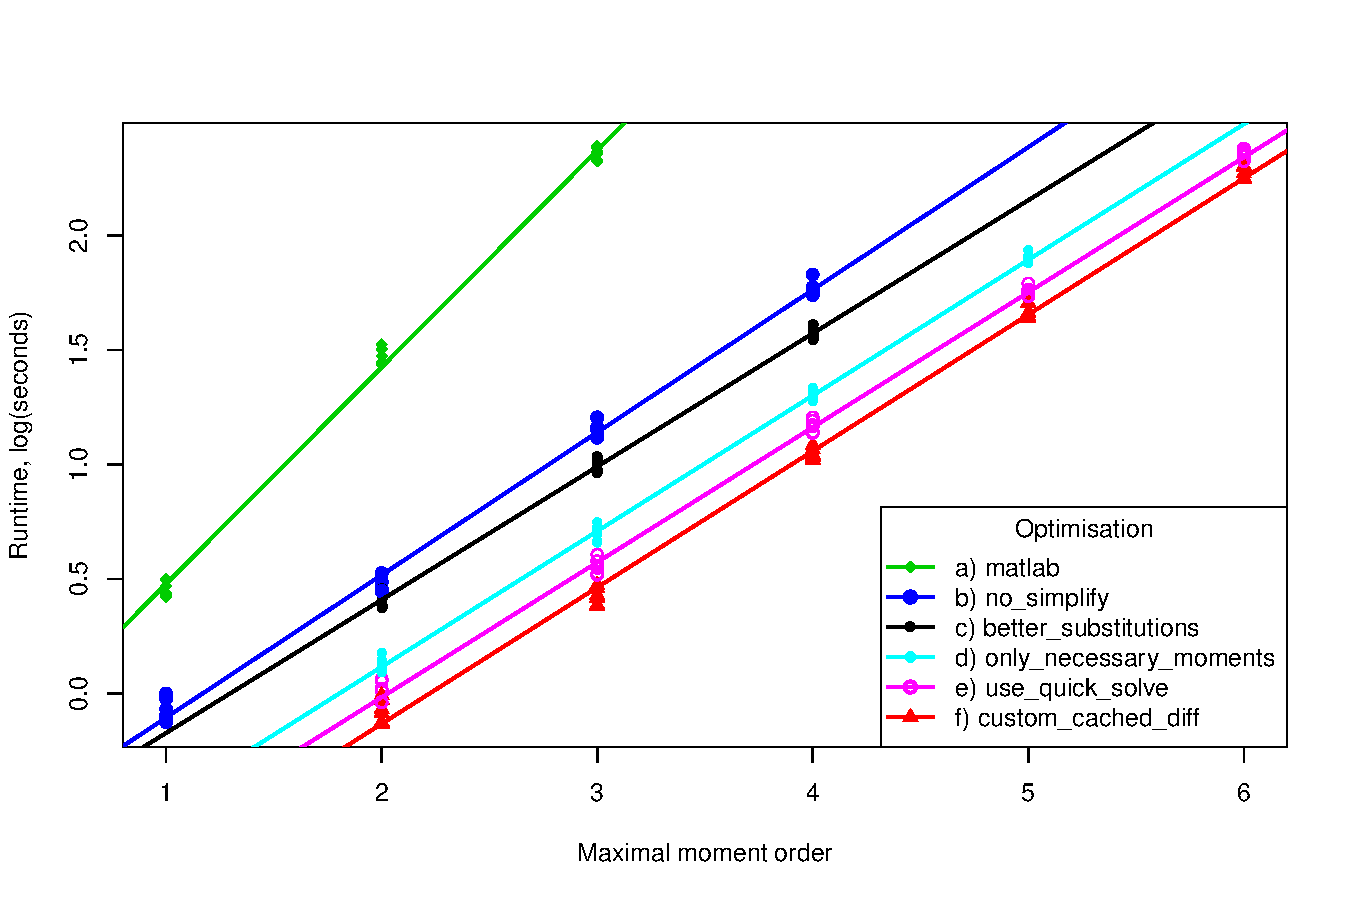
\includegraphics[width=1.0\textwidth{}]{../figure_mea_speed/mea_speed.pdf}
\caption{\emph{Cumulative performance improvement of symbolic calculations resulting from optimisation}.
The processing time for computing log-normal closure on \pft{} model with different maximal moment orders were measured for original Matlab implementation (a) and different optimisations (b$-$f).
In a first place, the calls to \texttt{sympy.simplify()} where removed (b). 
Then, \texttt{sympy.xreplace()} was used instead of \texttt{sympy.substitute()} (c). 
Generating an $(n-s) \times (n_2-s + 1)$ matrix (d), as opposed to an $(n-s) \times (n-s + 1)$ one, also increase speed (see main text).
Implementing a simplified equation solver instead of using \texttt{sympy.solve()} also resulted in a significant speed-up (e). Finally, caching (memorisation) \texttt{sympy.diff()} allowed even better performance.
The time complexity appears exponential ($O(2^n)$, where $n$ is the maximal moments order) in every case, 
Interestingly, the slopes between, a ($0.95$) and c ($0.58$), and b ($0.62$) and c were significantly different ($p-value <10^{-15}$ and $p-value = 3 \times 10^{-4}$, respectively; t-test on the slopes of the linear regression). 
No significant difference was found between the slopes of the subsequent optimisations (c$-$f). 
However, the intercepts were significantly smaller between each consecutive optimisations after c) ($p-value < 10^{-6}$ for all; t-test on the intercepts of the linear regression).
Nine replicates were performed on the same CPU. For optimisation c$-$f, values corresponding to maximal order moments lower than two were removed because of the inherent inaccuracy in measuring very short durations}
\label{fig:mea_speed}
\end{figure}

\quentintodo[inline]{Simplify this, move out the specific details to your individual report, it is enough to give just the overview here.}

The first step involved removing the expression simplification heuristic.
In the original code\footnote{both from the publication and last year's MSc project}, the right-hand-side equations were simplified in order to produce shorter text file results.
However, this was slow and did not benefit subsequent simulations and inference.
For large expressions, simplification had also had an large memory footprint and was likely to fail.
This optimisation significantly improved the scalability of the method (see fig.~\ref{fig:mea_speed}, b).

The next bottleneck was the choice of substitution functions.
As a part of \gls{mea}, it is necessary to replace raw moment symbols by expressions depending on central moments.
Performing substitution can be done using the \texttt{substitute()} function from \sympy, but this is designed to substitute expressions by other expressions.
In most cases, we only had to substitute atomic symbols by expression.
For this purpose, the  \texttt{xreplace()} function was a much more appropriate alternative which resulted in a better scalability (see fig.~\ref{fig:mea_speed}, c).

In the original implementation, a matrix of central moment expression of size $(n-s) \times (n-s + 1)$ is directly generated when the default closure is applied.
However, when using a parametric closure, a matrix of size $(n_2-s) \times (n_2-s + 1)$, where $n_2={{s+o-2 \mathbf{+1}} \choose {s}} -1$, was generated.
The $n_2 - n$ rows corresponding to higher-order moments have then to be deleted.
In contrast, out implementation generates a $(n-s) \times (n_2-s + 1)$ matrix regardless of the closure method.
In addition to improve code readability, consistency and flexibility \footnote{see QG's individual report}, this improved overall performance (fig.~\ref{fig:mea_speed}, d) for cases where closure is applied while keeping the default closure computation fast.

Another simple way to improve computation time was to remove calls to the function \texttt{solve()} which was only used in straightforward cases (\eg{} solving: $a + 2b = c$ for $a$).
It was therefore much more efficient (fig.~\ref{fig:mea_speed}, e) to use simple arithmetic to find solution.

Finally, partial derivation of expression over several variables and order is extensively performed during the approximation.
Generally, these type of differentiations can be simplified several differentiation of first order:
\begin{equation}
\frac{\partial{} ^ 2 f(x,y)}{\partial x \partial y}  =
\frac{\partial{} \frac{\partial{} f(x,y)}{\partial x}}{\partial y} =
\frac{\partial{} \frac{\partial{} f(x,y)}{\partial{} y}}{\partial{} x}
\end{equation}
One advantage, is that, when needing to calculate two derivatives such as:  $\frac{\partial{} ^ 2 f(x,y)}{\partial{} x \partial{} y}$ and $\frac{\partial{} ^ 2 f(x,y)}{\partial{} x^2}$, 
one can precompute $\frac{\partial{} f(x,y)}{\partial{} x}$ and use it for both calculation.
In our implementation, we have use a procedure known as \emph{memorisation} which, briefly, permits to store the results of a function call in an associative array.
Then, the next time this function is called with the same arguments, it will return the stored results instead of recomputing it.
This also resulted in an overall performance improvement (fig.~\ref{fig:mea_speed}, f).

In conclusion, reorganising, profiling and rewriting the code resulted in incremental significant performance improvements of symbolic computations in \means{} compared to the original \mat{} code.
For instance, with the same \pft{} system and closure method, 
we predict that computation up to \gls{ode}s up $8^{th}$ order will take 44 minutes with \means{} and as much as 128 days with the original implementation.\quentintodo{Add a number saying how long it would have taken for the first iteration of optimisation as well.}
These improvement have allowed us to explore the performance of MEA in higher depth, and will hopefully contribute to make \gls{mea} realistically usable for systems with more species and reactions.

\subsection{Moment Expansion Closure}

In \gls{mea} the temporal derivative of each central moment of order $n$ is expressed in terms of moment of order $n+1$.
For this reason, it is necessary to ``close'' the expansion by providing a closed form for the higher order moments.
In the original work \cite{ale_general_2013}, higher order central moments are assumed null. 
This is a strong and not necessarily valid assumption. 

Parametric probability distribution can be used to express moment of arbitrary orders. 
For instance, a multivariate normal distribution is parametrised only by means (\emph{i.e } first order raw moment)
and a covariance matrix (\emph{i.e.} second order central moments). 
As a consequence, it is possible to express any arbitrary moment from means, variances and covariances. 
A promising area of research involves closing moment expression by parametric forms of highest order central moments instead
of assuming them to be null.
Preliminary work \todo{cite Eszter, unpublished} suggests that using a parametric distributions for \gls{mea}
In addition, Ale \emph{et al.} predicted that higher maximal moment order would necessarily result in better approximation \cite{ale_general_2013}.
closure could greatly improve approximation.
The dramatic improvement in performance compared to the original code and implementation of parametric closures made it possible to verify both of these claims.

Figure~\ref{fig:max_order_and_closure_on_distance} shows the effect of increasing maximal moment order and different type of closures.
The \pft system, with parameters from \cite{ale_general_2013}, was investigated.
For normal and scalar closures, as expected, the approximation globally improves with maximal moment order (reduced distance to \gls{gssa}).
However, for 7$~{th}$ order, the scalar closure had an increased distance, and solving normal closures \gls{ode}s was not possible.
Note that for even maximal moment orders, normal and scalar are rigorously equal.
This is expected since normal distribution is symmetrical (\emph{i.e.} odd central moments are always zero).

In contrast, log$-$normal closures are fitting to the ground through trajectory well for maximal moment order of three,
but the approximation gets less and less accurate for higher maximal order moments.
A deeper look at the trajectories indicate that, in this latter case,
oscillations are damping too quickly (fig.~\ref{fig:max_order_and_closure_on_distance}b).
Interestingly for even maximum moment order log$-$normal closures generated \gls{ode}s which,
despite our efforts, could not be numerically solved.

Finally, for this system and parameter set, univariate and multivariate distributions closures were very similar.
For other systems such as \emph{hes1}, it was advantageous to model covariance (data not show).

This results indicates that the quality of the approximation depends both on the type of closure, on the maximal moment order and on their interaction. This makes it difficult to \emph{a priori} define which closure and maximal moment order should be used for a given system.

\begin{figure}

\includegraphics[width=1.0\textwidth]{../pipeline/task-output/FigureP53Summary/FigureP53Summary-pdf-7.pdf}
\includegraphics[width=1.0\textwidth]{../pipeline/task-output/FigureP53Simple/FigureP53Simple-pdf-7.pdf}
%~
\caption{\emph{Effect of different closure methods and maximal moment order on simulation accuracy}.
The \pft system was modelled using \gls{mea} with five types of closure and for maximal moment order up to seven.
Resulting trajectories were all compared to an average of 5000 \gls{gssa} simulations using sum of square distance (a).
Distance is in log scale.
For illustration purposes, complete trajectories of a single species (\pft) for max order three and seven are shown (b).
Black lines indicate the average of \gls{gssa} simulations. Missing points (b) and lines (a) indicate solver failure
TODO(see failure section.)}

\label{fig:max_order_and_closure_on_distance}
\end{figure}

\subsection{Inference}
Inference uses a distance method to infer parameter values by exploring the parameter space and comparing the distance between inferred system behaviour with experimental data. 

In order to study the performance of the inference method in \means, we used "sum of squares" distance method and p53 model. 
Due to the lack of experimental concentrations of the species, the averaged concentration change through time from $5000$ \gls{gssa} are used as the observed trajectories. 
With full variability for all the parameters in the p53 model, and starting values equal to the values from \cite{gillespie_general_1976}, it is expected that the inference method would return the same values as the starting values. 
To visualise how the system explored the multi-dimensional parameter space, we studied the cross-section for all possible pairs of parameters. \sisitodo{find the 7 dimensional figure} 
Unexpectedly, trajectories simulated with the true parameter values are distant from the \gls{gssa} trajectories, forcing the system to follow the distant gradient and infer incorrect parameter values. This result implies inference method is may not infer the right parameter set. 

To confirm if the inference method can find the global minima, we recorded the inferred parameter values using one pair of parameters at a time for all possible pairs of parameters, and used these values as the starting values to re-generated the distance landscape (see Figure 5 \sisitodo{check if it's the right number}). 
Here, we explicitly allow $c_2$ and $c_6$ values to vary, but keep other parameter values the true values, because $c_2$ and $c_6$ with variability in their values are able to produce an almost perfect match with the \gls{gssa} trajectories of all species (data not shown). 
If the inference method was correct, the starting point in the distance landscape would already have a low distance, and the end point should overlap with the starting point, i.e. the true values of $c_2$ and $c_6$.
However, the resulting distance landscape figures and trajectories for each species clearly indicate that the starting point is not the global minima, because: Firstly, the trajectories in the distance landscape shows the starting point can be distant from the minima; Secondly, the possible range for $c_6$, despite the maximal order for \gls{mea}, is mostly more than 10 times larger than the true value; Thirdly, the trajectories for all the species in the p53 model sometime demonstrate misfit between the optimal trajectory obtained from inference and the "observed trajectory" from \gls{gssa}. 

Based on these results, we can conclude that the inference method here is inaccurate.
\begin{figure}
\centering
    \begin{subfigure}
    \includegraphics[width=0.2\textwidth]{{../pipeline/task-output/SampleMultidimensionInferenceFigure/SampleMultidimensionInferenceFigure-pdf-1-scalar-True-90.0_0.002_1.704_1.1_0.93_0.96_0.7822-ode15s--90.0_0.002_1.704_1.1_0.93_0.96_0.7822-sum_of_squares-5000}.pdf}
    \end{subfigure}
    \begin{subfigure}
    \includegraphics[width=0.2\textwidth]{{../pipeline/task-output/SampleMultidimensionInferenceFigure/SampleMultidimensionInferenceFigure-pdf-2-scalar-True-90.0_0.002_1.704_1.1_0.93_0.96_0.7822-ode15s--90.0_0.002_1.704_1.1_0.93_0.96_0.7822-sum_of_squares-5000}.pdf}
    \end{subfigure}
    \begin{subfigure}

    \includegraphics[width=0.2\textwidth]{{../pipeline/task-output/SampleMultidimensionInferenceFigure/SampleMultidimensionInferenceFigure-pdf-3-scalar-True-90.0_0.002_1.704_1.1_0.93_0.96_0.7822-ode15s--90.0_0.002_1.704_1.1_0.93_0.96_0.7822-sum_of_squares-5000}.pdf}
    \end{subfigure}
    \begin{subfigure}
    \includegraphics[width=0.2\textwidth]{{../pipeline/task-output/SampleMultidimensionInferenceFigure/SampleMultidimensionInferenceFigure-pdf-4-scalar-True-90.0_0.002_1.704_1.1_0.93_0.96_0.7822-ode15s--90.0_0.002_1.704_1.1_0.93_0.96_0.7822-sum_of_squares-5000}.pdf}
    \end{subfigure}
    \begin{subfigure}
    \includegraphics[width=0.2\textwidth]{{../pipeline/task-output/SampleMultidimensionInferenceFigure/SampleMultidimensionInferenceFigure-pdf-5-scalar-True-90.0_0.002_1.704_1.1_0.93_0.96_0.7822-ode15s--90.0_0.002_1.704_1.1_0.93_0.96_0.7822-sum_of_squares-5000}.pdf}
    \end{subfigure}

\caption{\emph{Distance landscape at different maximal orders for p53 model.} In the landscape, the warmer the colour, the more distant the inferred trajectories are from the \gls{gssa} trajectories. 
The \gls{gssa} trajectories are generated using the new parameter values labelled as \emph{start}. Among seven parameters, only the values for $c_2$ and $c_6$ are inferred, with starting values inferred from inference using the true values.} 
\label{fig:parameter_inference_landscape}
\end{figure}

\begin{figure}
\centering
    \begin{subfigure}
    \includegraphics[width=0.6\textwidth]{{../pipeline/task-output/FigureInferenceStartEndSSA/FigureInferenceStartEndSSA-1-scalar-c2-1.7040-c6-0.7822}.pdf}
    \end{subfigure}
    \begin{subfigure}
    \includegraphics[width=0.6\textwidth]{{../pipeline/task-output/FigureInferenceStartEndSSA/FigureInferenceStartEndSSA-2-scalar-c2-1.7040-c6-0.7822}.pdf}
    \end{subfigure}
    \begin{subfigure}    
    \includegraphics[width=0.6\textwidth]{{../pipeline/task-output/FigureInferenceStartEndSSA/FigureInferenceStartEndSSA-3-scalar-c2-1.7040-c6-0.7822}.pdf}
    \end{subfigure}
    \begin{subfigure}   
    \includegraphics[width=0.6\textwidth]{{../pipeline/task-output/FigureInferenceStartEndSSA/FigureInferenceStartEndSSA-4-scalar-c2-1.7040-c6-0.7822}.pdf}
    \end{subfigure}
    \begin{subfigure}
    \includegraphics[width=0.6\textwidth]{{../pipeline/task-output/FigureInferenceStartEndSSA/FigureInferenceStartEndSSA-5-scalar-c2-1.7040-c6-0.7822}.pdf}
    \end{subfigure}
\end{figure}
\caption{\emph{Trajectories for each species in p53 model using different maximal orders.} 
Three trajectories are shown for each species. 
The starting trajectories are simulated using the starting values are indicated above the trajectories, with $c_2$ and $c_6$ inferred using \emph{sum of squares} distance method. 
Both the optimal and the \gls{gssa} trajectories are generated based on the end point in correspondent distance landscape in Figure 5.} 
\label{fig:parameter_inference_trajectories}
\end{figure}

\newpage{}
\section{Conclusion} \label{conclus}

\newpage{}
\bibliography{report.bib}{}
\bibliographystyle{ieeetr}

\newpage{}
\begin{appendices}
\section{\\Tutorials} \label{tutorials}

\end{appendices}
   
\end{document}
